% yaml_unicef_workflow.tex
% UNICEF-specific workflow diagram showing real use cases
% Author: João Pedro Azevedo
% Date: December 2025

\documentclass[tikz,border=10pt]{standalone}
\usepackage{tikz}
\usetikzlibrary{shapes.geometric, arrows.meta, positioning, fit, backgrounds, calc}

\begin{document}

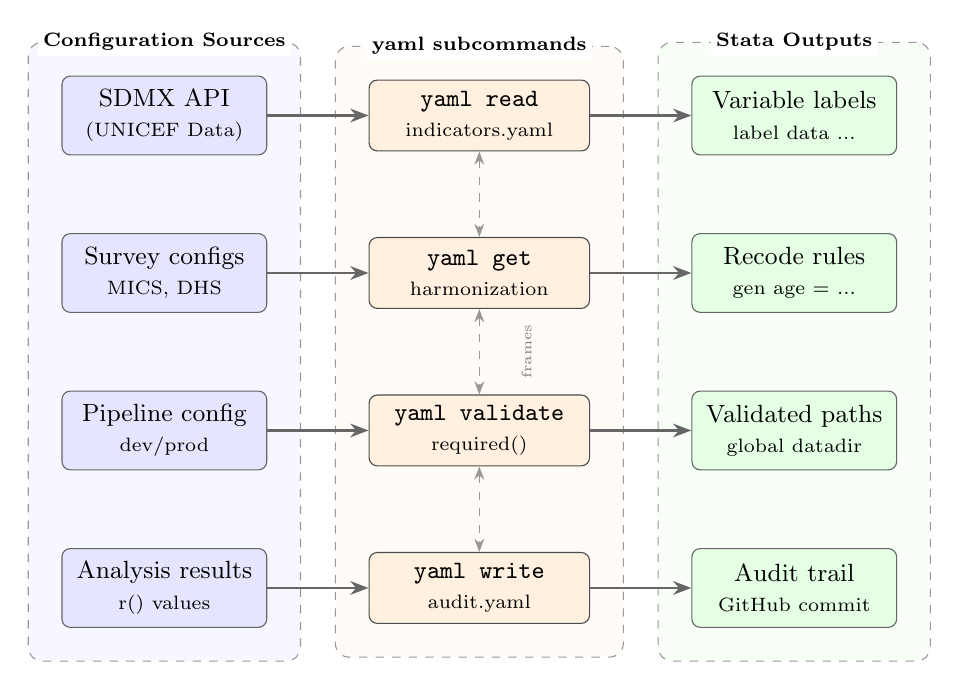
\begin{tikzpicture}[
    % Source style
    sourcebox/.style={
        rectangle, 
        rounded corners=3pt,
        draw=black!60, 
        fill=blue!10,
        minimum width=2.6cm, 
        minimum height=1cm,
        font=\small,
        align=center
    },
    % Process style
    processbox/.style={
        rectangle, 
        rounded corners=3pt,
        draw=black!70, 
        fill=orange!12,
        minimum width=2.8cm, 
        minimum height=0.9cm,
        font=\small,
        align=center
    },
    % Output style
    outputbox/.style={
        rectangle, 
        rounded corners=3pt,
        draw=black!60, 
        fill=green!10,
        minimum width=2.6cm, 
        minimum height=1cm,
        font=\small,
        align=center
    },
    arrow/.style={
        ->,
        >=Stealth,
        thick,
        black!60
    },
    groupbox/.style={
        rectangle,
        rounded corners=5pt,
        draw=black!40,
        dashed,
        inner sep=10pt
    },
    grouplabel/.style={
        font=\scriptsize\bfseries,
        fill=white,
        inner sep=2pt
    }
]

% === Row 1: SDMX Metadata Flow ===
\node[sourcebox] (sdmx) at (0, 4) {SDMX API\\{\scriptsize(UNICEF Data)}};
\node[processbox] (yaml1) at (4, 4) {\ttfamily yaml read\\{\scriptsize indicators.yaml}};
\node[outputbox] (labels) at (8, 4) {Variable labels\\{\scriptsize label data ...}};

\draw[arrow] (sdmx) -- (yaml1);
\draw[arrow] (yaml1) -- (labels);

% === Row 2: Harmonization Flow ===
\node[sourcebox] (surveys) at (0, 2) {Survey configs\\{\scriptsize MICS, DHS}};
\node[processbox] (yaml2) at (4, 2) {\ttfamily yaml get\\{\scriptsize harmonization}};
\node[outputbox] (recode) at (8, 2) {Recode rules\\{\scriptsize gen age = ...}};

\draw[arrow] (surveys) -- (yaml2);
\draw[arrow] (yaml2) -- (recode);

% === Row 3: Pipeline Config Flow ===
\node[sourcebox] (config) at (0, 0) {Pipeline config\\{\scriptsize dev/prod}};
\node[processbox] (yaml3) at (4, 0) {\ttfamily yaml validate\\{\scriptsize required()}};
\node[outputbox] (paths) at (8, 0) {Validated paths\\{\scriptsize global datadir}};

\draw[arrow] (config) -- (yaml3);
\draw[arrow] (yaml3) -- (paths);

% === Row 4: Output Flow ===
\node[sourcebox] (results) at (0, -2) {Analysis results\\{\scriptsize r() values}};
\node[processbox] (yaml4) at (4, -2) {\ttfamily yaml write\\{\scriptsize audit.yaml}};
\node[outputbox] (audit) at (8, -2) {Audit trail\\{\scriptsize GitHub commit}};

\draw[arrow] (results) -- (yaml4);
\draw[arrow] (yaml4) -- (audit);

% === Group boxes ===
\begin{scope}[on background layer]
    \node[groupbox, fit=(sdmx)(surveys)(config)(results), inner sep=12pt, fill=blue!3] (inputgroup) {};
    \node[groupbox, fit=(yaml1)(yaml2)(yaml3)(yaml4), inner sep=12pt, fill=orange!3] (statagroup) {};
    \node[groupbox, fit=(labels)(recode)(paths)(audit), inner sep=12pt, fill=green!3] (outputgroup) {};
\end{scope}

% === Group labels ===
\node[grouplabel] at (inputgroup.north) {Configuration Sources};
\node[grouplabel] at (statagroup.north) {yaml subcommands};
\node[grouplabel] at (outputgroup.north) {Stata Outputs};

% === Vertical connection: frames ===
\draw[<->, >=Stealth, dashed, black!40] (yaml1.south) -- (yaml2.north);
\draw[<->, >=Stealth, dashed, black!40] (yaml2.south) -- (yaml3.north);
\draw[<->, >=Stealth, dashed, black!40] (yaml3.south) -- (yaml4.north);
\node[font=\tiny, text=black!50, rotate=90] at (4.6, 1) {frames};

\end{tikzpicture}

\end{document}
